% questions.tex —— 1984 年·全国卷（文科） · 题目内容片段（无答案）
% 由 tools/generate_projects.py 依来源总账自 1984/1984_数学真题_文_试题.md 生成，勿手改（改源 MD 后重跑）


\begin{gktip}
\textbf{来源说明}：本卷为 1984 年全国统一命题的\textbf{文科数学}卷（同年另有独立的理科卷，两份试卷题目不同），单页扫描（原卷页码第 24 页），全卷共 17 题，其中第 1—5 题为选择题。题面不含答案（答案由本库独立推导）。原卷按左、中、右三栏分栏排版，本文按题号 1—17 顺序转录，题面文字未作改动。

\textbf{题面说明}：第 11、12 题为作图题（原卷只在题面下方留白供作图，未印图形）。第 15 题依原卷配图重绘为 TikZ 矢量图。

\textbf{源注}：第 8 题原卷只写明「实数 $m$」，未注明 $x$ 的取值范围；本库按题意取 $x$ 为实数（若允许 $x$ 为复数，则 $(m,x)$ 有无穷多组解），详见解析正文。纯文本提取会丢第 1 题数集 $Y$ 中的「$\pm$」号、弄乱第 3 题的根号与分数层次，本文均以页面图像为准转录。
\end{gktip}

\begin{question}
\gkti{1}数集 $X=\{(2n+1)\pi,\ n\text{\text{是整数}}\}$ 与数集 $Y=\{(4k\pm1)\pi,\ k\text{\text{是整数}}\}$ 之间的关系是\mbox{（　　）}

\begin{gkopts}(4)
\task A．$X\subseteq Y$
\task B．$X\supseteq Y$
\task C．$X=Y$
\task D．$X\ne Y$
\end{gkopts}

\end{question}
\begin{question}
\gkti{2}函数 $y=f(x)$ 与它的反函数 $y=f^{-1}(x)$ 的图象\mbox{（　　）}

\begin{gkopts}(2)
\task A．关于 $y$ 轴对称
\task B．关于原点对称
\task C．关于直线 $x+y=0$ 对称
\task D．关于直线 $x-y=0$ 对称
\end{gkopts}

\end{question}
\begin{question}
\gkti{3}复数 $\dfrac12-\dfrac{\sqrt3}{2}\mathrm i$ 的三角形式是\mbox{（　　）}

\begin{gkopts}(1)
\task A．$\cos\left(-\dfrac{\pi}{3}\right)+\mathrm i\sin\left(-\dfrac{\pi}{3}\right)$
\task B．$\cos\dfrac{\pi}{3}+\mathrm i\sin\dfrac{\pi}{3}$
\task C．$\cos\dfrac{\pi}{3}-\mathrm i\sin\dfrac{\pi}{3}$
\task D．$\cos\dfrac{\pi}{3}+\mathrm i\sin\dfrac{5\pi}{6}$
\end{gkopts}

\end{question}
\begin{question}
\gkti{4}直线与平面平行的充要条件是这条直线与平面内的\mbox{（　　）}

\begin{gkopts}(2)
\task A．一条直线不相交
\task B．两条直线不相交
\task C．任意一条直线都不相交
\task D．无数条直线不相交
\end{gkopts}

\end{question}
\begin{question}
\gkti{5}方程 $x^2-79x+1=0$ 的两根可分别作为\mbox{（　　）}

\begin{gkopts}(2)
\task A．一椭圆和一双曲线的离心率
\task B．两抛物线的离心率
\task C．一椭圆和一抛物线的离心率
\task D．两椭圆的离心率
\end{gkopts}

\end{question}
\begin{question}
\gkti{6}已知函数 $\log_{0.5}(2x-3)>0$，求 $x$ 的取值范围。

\end{question}
\begin{question}
\gkti{7}已知圆柱的侧面展开图是边长为 $2$ 与 $4$ 的矩形，求圆柱的体积。

\end{question}
\begin{question}
\gkti{8}已知实数 $m$ 满足 $2x^2-(2\mathrm i-1)x+m-\mathrm i=0$，求 $m$ 及 $x$ 的值。

\end{question}
\begin{question}
\gkti{9}求 $\lim\limits_{n\to\infty}\dfrac{(n^2+1)+(n^2+2)+\cdots+(n^2+n)}{n(n-1)(n-2)}$ 的值。

\end{question}
\begin{question}
\gkti{10}要排一张有 $6$ 个歌唱节目和 $4$ 个舞蹈节目的演出节目单，任何两个舞蹈节目不得相邻，问有多少种不同的排法（只要求写出式子，不必计算）。

\end{question}
\begin{question}
\gkti{11}画出方程 $y^2=-4x$ 的曲线。

\end{question}
\begin{question}
\gkti{12}画出函数 $y=\dfrac{1}{(x+1)^2}$ 的图象。

\end{question}
\begin{question}
\gkti{13}已知等差数列 $a$、$b$、$c$ 中的三个数都是正数，且公差不为零。求证它们的倒数所组成的数列 $\dfrac1a$、$\dfrac1b$、$\dfrac1c$ 不可能成等差数列。

\end{question}
\begin{question}
\gkti{14}把 $1-\dfrac14\sin^2 2\alpha-\sin^2\beta-\cos^4\alpha$ 化成三角函数的积的形式（要求结果最简）。

\Needspace{0.4\textheight}
\end{question}
\begin{question}
\gkti{15}如图，经过正三棱柱底面一边 $AB$，作与底面成 $30^\circ$ 角的平面，已知截面三角形 $ABD$ 的面积为 $32\ \mathrm{cm}^2$，求截得的三棱锥 $D-ABC$ 的体积。
\nopagebreak[4]
\begin{center}% 1984 年全国卷（文科）第 15 题：正三棱柱（底面三角形 A 在前、B 在右、C 在左，三条侧棱竖直），
% 经过底面一边 AB 作与底面成 30° 角的平面，截面为三角形 ABD，D 在过 C 的侧棱上；
% 顶面可见，故顶面三边画实线；底面后边 CB 与被后侧面遮住的截面边 DB 画虚线（按源卷布局）
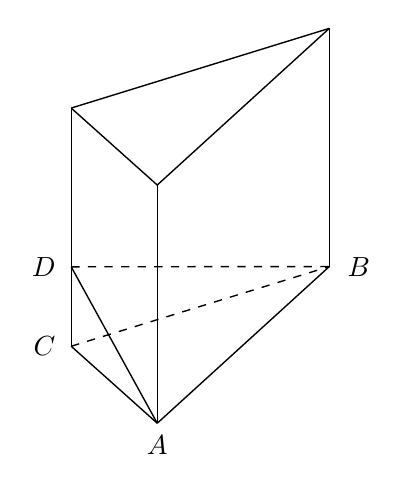
\begin{tikzpicture}[scale=1.15, line width=0.5pt,
  every node/.style={inner sep=1.5pt}]
  % 顶点坐标（按源卷布局手算：底面三顶点 + 各自正上方等高 H=2.63 的顶面三顶点）
  \coordinate (A)  at (0.95, 0);      % 底面前顶点
  \coordinate (B)  at (2.85, 1.73);   % 底面右顶点
  \coordinate (C)  at (0.00, 0.85);   % 底面左顶点
  \coordinate (A1) at (0.95, 2.63);   % 顶面前顶点（在 A 正上方）
  \coordinate (B1) at (2.85, 4.36);   % 顶面右顶点（在 B 正上方）
  \coordinate (C1) at (0.00, 3.48);   % 顶面左顶点（在 C 正上方）
  \coordinate (D)  at (0.00, 1.727);  % 侧棱 CC1 上一点，C 到 D 约为 C 到 C1 的 1/3
  % 被遮住的棱：底面后边 CB、截面边 DB
  \draw[dashed] (C) -- (B);
  \draw[dashed] (D) -- (B);
  % 可见的棱
  \draw (A) -- (B);
  \draw (A) -- (C);
  \draw (A) -- (A1);
  \draw (B) -- (B1);
  \draw (C) -- (C1);
  \draw (A1) -- (B1);
  \draw (A1) -- (C1);
  \draw (C1) -- (B1);
  % 截面三角形 ABD 在可见侧面 ACC1A1 内的边 AD
  \draw (A) -- (D);
  % 标注
  \node[anchor=north] at (0.95,-0.08) {$A$};
  \node[anchor=west] at (3.00,1.73) {$B$};
  \node[anchor=east] at (-0.12,0.85) {$C$};
  \node[anchor=east] at (-0.12,1.727) {$D$};
\end{tikzpicture}
\end{center}
\nopagebreak[4]
\end{question}
\begin{question}
\gkti{16}某工厂 1983 年生产某种产品 $2$ 万件，计划从 1984 年开始，每年的产量比上一年增长 $20\%$。问从哪一年开始，这家工厂生产这种产品的年产量超过 $12$ 万件（已知 $\lg 2=0.3010$，$\lg 3=0.4771$）。

\end{question}
\begin{question}
\gkti{17}已知两个椭圆的方程分别是 $C_1:x^2+9y^2-45=0$，$C_2:x^2+9y^2-6x-27=0$。

（1） 求这两个椭圆的中心、焦点的坐标；

（2） 求经过这两个椭圆的交点且与直线 $x-2y+11=0$ 相切的圆的方程。

\end{question}